\documentclass[a4paper]{ctexart}
\usepackage{geometry}
\usepackage{listings}
\usepackage{hyperref}
\usepackage{graphicx}
\geometry{left=2cm,right=2cm,top=2.5cm,bottom=2.5cm}

\author{严春伟}
\title{隐式马尔科夫模型在信息提取中的应用}
\begin{document}
    \maketitle

\section{前言}
\par 信息提取(Information Extraction),也就是从非结构的数据中提取出结构化数据,如从自然语言文本中提取出相关的信息,然后存储到结构化的数据库中。
\par 如何能够从庞大的互联网自然语言文本化的数据中提取出我们所感兴趣的数据一直是自然语言处理的重点研究方向,也是我比较感兴趣的方面。
\par 隐马尔科夫模型(Hidden Markov model)在传统的自然语言处理(如统计机器翻译、以及语音识别方面)用的非常成熟,而将HMM用于IE还是一个比较新的尝试。 目前,大部分IE的实现仍旧需要建立模板,通过模板从自然语言文本中提取数据,如果人工建立模板的话,是一个非常繁琐的事情,而且模板永远是滞后的。 通过HMM模型以及机器学习的方式来训练出模板是一件非常有前景的事情。 前人通过HMM模型来进行一些相对简单的信息提取实验,实现的模型的精度甚至超出了人工的水平。可见HMM(以及条件随机场)等在IE领域前途非常广阔。
\par 隐马尔科夫模型是一种统计学习模型,可以用于标注问题。隐马尔科夫模型在序列化的数据的处理中有比较成熟的应用,如:
\begin{itemize}
\item 语音识别
\item 自然语言处理
\item 生物信息
\item 模式识别
\end{itemize}
\par
本文将会论述隐马尔科夫的基本问题,如定义,解决问题,基本算法等,此外,本文还会论述HMM在IE方面的一个应用的思想。

\section{基本概念}
\subsection{定义}
\paragraph{隐马尔科夫模型(HMM)} 描述一个隐藏的马尔科夫链生成不可观察的状态(state)随机序列,在由各个状态生成一个观测而产生观测随机序列的过程。
\par
HMM的确定因素:
\begin{enumerate}
\item 初始状态分布 $\pi$
\item 状态转移概率分布 $A$
\item 观测概率 $B$
\end{enumerate}

\paragraph{隐马尔科夫的要素}
\begin{enumerate}
\item N,表示模型中的状态数目
\item M,表示模型中每个状态不同的观察符号
\item A,状态转移概率分布。$A=\{a_{ij}\}$
    \begin{equation}
    a_{ij} = P(q_t = S_j | q_{t-1} = S_j) \quad 1\le j\le N     
    \end{equation}
\item B,观察字符在状态j时的概率分布,$B=\{b_j(k)\}$,其中
    \begin{equation}
    b_j(k) = P(v_k|q_t = S_j) \quad 1\le j \le N, 1 \le k \le M
    \end{equation}
\end{enumerate}

\subsection{三个基本问题}
\begin{enumerate}
    \item 给定一个模型$\gamma = {N,M,A,B,\pi}$,如何高效地计算某一输出字符序列$O= O_1 O_2 \cdots \O_n$,如何找到产生这一序列概率的最大的概率序列.
    \item 给定一个模型$\gamma = {N,M,A,B,\pi}$和一个输出字符序列$O=O_1O_2\cdots O_n$,如何调整模型的成熟使得产生这一序列的概率最大的状态系列$\varrho = s_is_j\cdots s_T$.
    \item 给定一个模型$\gamma = {N,M,A,B,\pi}$和一个输出字符序列$O=O_1O_2\cdots O_n$, 如何调整模型的参数使得产生这一序列的概率最大.
\end{enumerate}
\subsection{条件性假设}
\begin{enumerate}
    \item t 时刻的状态$q_t = s_i$只依赖于$t-1$时刻的状态$q_{t-1} = s_j$,即
        \begin{equation}
            P(q_1|q_{t-1}\cdots q_1, \gamma) = P(q_t|q_{t-1},\gamma)
        \end{equation}
    \item t 时刻生成的值$b_i(O_t)$ 只依赖与t时刻的状态$q_t=s_i$,即
        \begin{equation}
            P(O_1O_2\cdots O_T | q_1 q_2 \cdots q_T, \gamma) = \Pi_{t=1}^{T}P(O_{t}|q_{t})
        \end{equation}
    \item 状态与具体的时间无关
        \begin{equation}
            P(q_i | q_{i-1}, \gamma) = P(q_j | q_{j-1}, \gamma)
        \end{equation}
\end{enumerate}

\section{HMM的概率计算}
\par 假如给定一个评论问题,给定一个模型$\gamma$和一个观察序列$O=O_1O_2\cdots O_T$,如何计算由这一模型产生观察序列的概率.
\par 由于状态是不可见的,要计算观察序列的概率,必定需要回到状态. 不妨假设其中一个状态序列是
\begin{equation}
    \varrho = q_1 q_2 \cdots q_T
\end{equation}
\par 其中$q_1$为初始状态,则此时序列O的概率为
\begin{equation}
    P(O|\varrho, \gamma) = \Pi_{t=1}^{T}P(O_t|q_t,\gamma) = \Pi_{t=1}^{T}b_{q_t}(O_{t}) 
\end{equation}
\par 如此,知道在某一特定状态下产生观察序列的概率,最简单的方式就是利用穷举法,但是其复杂度达到了$2TN^T$,其中N为模型中的状态数,T为观察序列的长度.

\par HMM模型是一个比较成熟的模型,在漫长的发展中,已经有许多成熟的方法,本文将会简单介绍比较经典的forward 和 backward 算法.

\subsection{forward 算法}
\par forward 以及后面的 backward 算法的核心都是定义了一个核心的公式形式,通过这个公式形式完成递推迭代.
\par 定义 forward 变量$\alpha_{t}(i)$为
\begin{equation}
    \alpha_{t}(t) = P(O_1 O_2 \cdots O_t, q_t = s_i | \gamma)
\end{equation}
\par 那么递推起来就是
\begin{eqnarray*}
    \alpha_{j}(t+1)     &   =   &   P(O_1 O_2 \cdots O_{t+1}, q_{t+1} = s_{j}| \gamma)\\
    &   =   &   \left[ \sum_{i=1}^{N}\alpha_{i}(t) a_{ij} \right]b_{j}(O_{t+1})\\
\end{eqnarray*}
\par 利用这个特殊的递推形式,最终的概率为
\begin{equation}
    P(O|\gamma) = \sum_{i=1}^{N} \alpha_{T}(i)
\end{equation}
\par forward 算法的计算量是 $N^{2}T$,远小于穷举法的$2TN^T$.

\subsection{backward 算法}
\par backward 算法与forward 算法思想基本一致,特性也相同
\par 其核心递推变量:
\begin{equation}
    \beta_{t}(i) = P(O_{t+1} O_{t+2} \cdots O_{T} | q_{t} = s_{i}, \gamma)
\end{equation}
\begin{equation}
    \beta_{i}(j) = \sum_{j=1}^{N} a_{ij}b_{j}(O_{t+1})\beta_{t+1}(j), \quad t=T-1, T-2, \cdots, 1, \quad 1\le i \le N.
\end{equation}

\subsection{Viterbi 算法}
\par 给定一个解码问题,从$N^T$个可能的状态序列中找到一个''最优''的状态序列,其中$N$是HMMs模型 的状态个数,T是观察序列的长度。
\par 定义一个变量$\gamma_i(i)$表示给定观察序列O和模型$\gamma$条件下,在t时刻,状态为$q_t = s_t$的概率:
\begin{equation}
    \gamma_{i}(i) = P(q_t = s_t | O, \gamma)
\end{equation}
\par 可以用之前介绍的 forward \quad  backward 算法来表示:
\begin{equation}
    \gamma_t(i) = \frac{\alpha_{t}(i) \beta_t(i)}
    {P(O|\gamma)}
    = \frac{\alpha_t{(i)} \beta_{t}(i)}
    {\sum_{t=1}^{N}\alpha_{t(i)}\beta_{t}(i)}
\end{equation}
\par 如此,利用$\gamma_{t}(i)$就可以找出t时刻单个概率最大的状态$q_{t}$:
\begin{equation}
    q_t = arg\max_{1 \le i \le N}{\gamma_{i}(i)}, 1\le t \le T
\end{equation}

\par Viterbi算法在实现中,最核心的一个思想就是类似图理论中最短路径,根据动态规划理论,最优路径的特性:如果最优路径在时刻t通过节点$i_{t}^{*}$,那么这一路径从节点$i_{t}^{*}$到终点$i_{T}^{*}$的部分路径,对于从$i_{t}^{*}$到$i_{T}^{*}$的所有可能的部分路径来说,必须是最优的。
\par Viterbi算法运行时,会按照步骤动态搜索和保存局部最优的路径,直至最终最优路径生成。计算复杂度为$NT^2$。

\section{HMM在IE中的一种应用思路}
\par 现在有一个任务,有一大堆论文,需要从论文的头部提取出作者名称、邮箱地址、地址、单位、年份等信息。
\par 常规的做法是采用正则表达式人工构建模板,或者利用简单机器学习的方式,构建硬性组合模板。前者是工作繁琐;后者尽管降低了人工负担,但适应性比较弱。
\par 由于论文头部信息的格式千变万化,但是不变的是内容。人工如何去识别,那就是通过理解的方式。那么如何让机器理解论文头部的内容,从语义的层次来识别出论文头不同的部分,这就是HMM模型的应用之处。
\par 设定HMM隐含的状态为相应的标注标签,如:标题、作者、邮箱地址等。而观测就是具体的内容。我们的目标是训练出一个模型,能够通过处理了论文头的内容,还原出最优可能的状态序列。
\par 首先需要进对数据集进行标注,然后进行模板训练
\begin{equation}
    \hat{P}(q \rightarrow q') = 
        \frac{c(q \rightarrow q')} {\sum_{\delta \in Q}c(q \rightarrow s)}
\end{equation}
\begin{equation}
    \hat{P}(q \uparrow \delta) = 
        \frac{c(q \uparrow \delta)}
        {\sum_{\rho \in \sum}c(q \uparrow p)}
\end{equation}
\par 其中$c(q \rightarrow q')$表示从状态$q$转移到状态$q'$的数量。
\par $c(q \uparrow \delta)$ 表示从状态$q$得到观测$\delta$的数量。
\par 通过这些,学习出HMM的模型$\gamma$,然后就可以进行标注了。传入一个论文头,HMM模型转化出其状态序列,通过状态序列,就可以得到各种信息了。

\begin{figure}[]
    \centering
    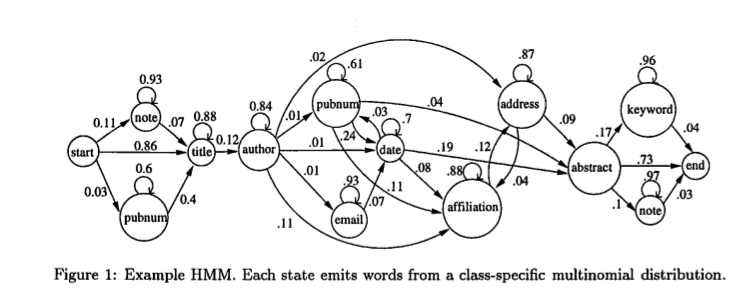
\includegraphics[height=150pt]{hmm.png}
    \caption{状态转移示意图}
    \label{fig:hmm}
\end{figure}

\begin{thebibliography}{sotief}
        \bibitem{learn-method} 李航,统计学习方法,清华大学出版社.2012
        \bibitem{crf}基于CRFs的中文分词算法研究与实现
        \bibitem{IE} Andrew McCallum, Dayne Freitag, and Fernando Pereira, Maximum Entropy Markov Models for Information Extraction and Segmentation
\end{thebibliography}

\end{document}
